\documentclass[tikz,border=10pt]{standalone}
\usepackage{tikz}
\usetikzlibrary{shapes.geometric, arrows.meta, positioning}

\tikzset{
    block/.style={rectangle, draw, fill=blue!20, text width=5em, text centered, rounded corners, minimum height=4em},
    line/.style={draw, thick, -Stealth}
}

\begin{document}
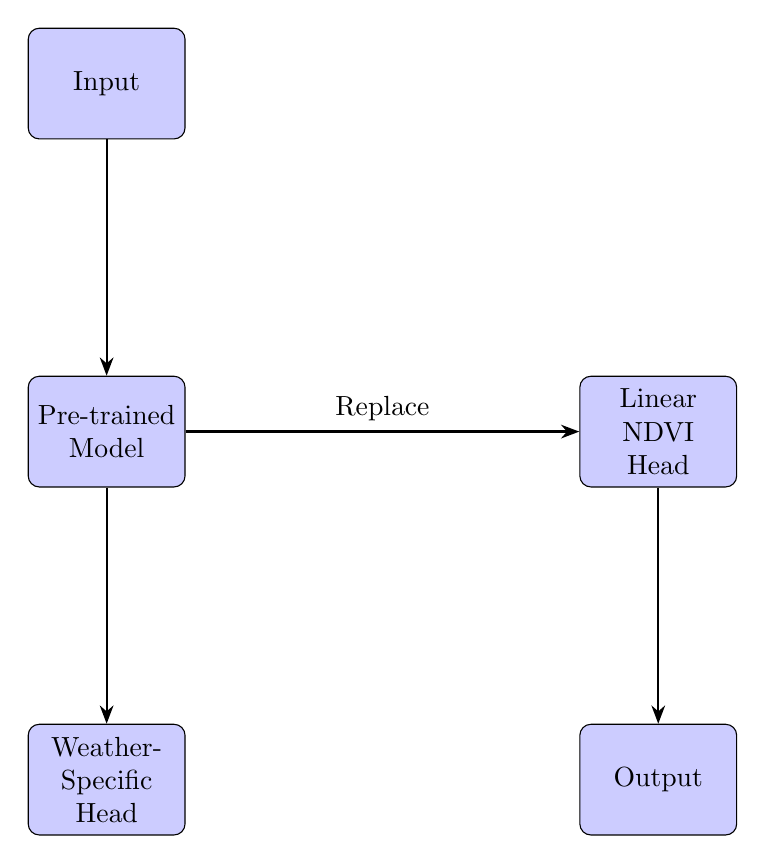
\begin{tikzpicture}[node distance=2cm]
    % Input Layer
    \node[block] (input) {Input};
    
    % Pre-trained Model
    \node[block, below=of input, yshift=-1cm] (pretrained_model) {Pre-trained Model};
    
    % Weather-Specific Head
    \node[block, below=of pretrained_model, yshift=-1cm] (weather_head) {Weather-Specific Head};
    
    % Linear NDVI Head
    \node[block, right=of pretrained_model, xshift=3cm] (ndvi_head) {Linear NDVI Head};
    
    % Output Layer
    \node[block, below=of ndvi_head, yshift=-1cm] (output) {Output};
    
    % Connections
    \draw [line] (input) -- (pretrained_model);
    \draw [line] (pretrained_model) -- (weather_head);
    \draw [line] (pretrained_model.east) -- node[anchor=south] {Replace} (ndvi_head.west);
    \draw [line] (ndvi_head) -- (output);
\end{tikzpicture}
\end{document}